
Templates can also be used to implement polymorphism. However, they don’t rely on the factoring of common behavior in base classes. Instead, the commonality is implicit in that the different “shapes” of an application must support operations using common syntax (i.e., the relevant functions must have the same names). Concrete classes are defined independently from each other (see Figure 18.2). The polymorphic power is then enabled when templates are instantiated with the concrete classes.

\begin{center}
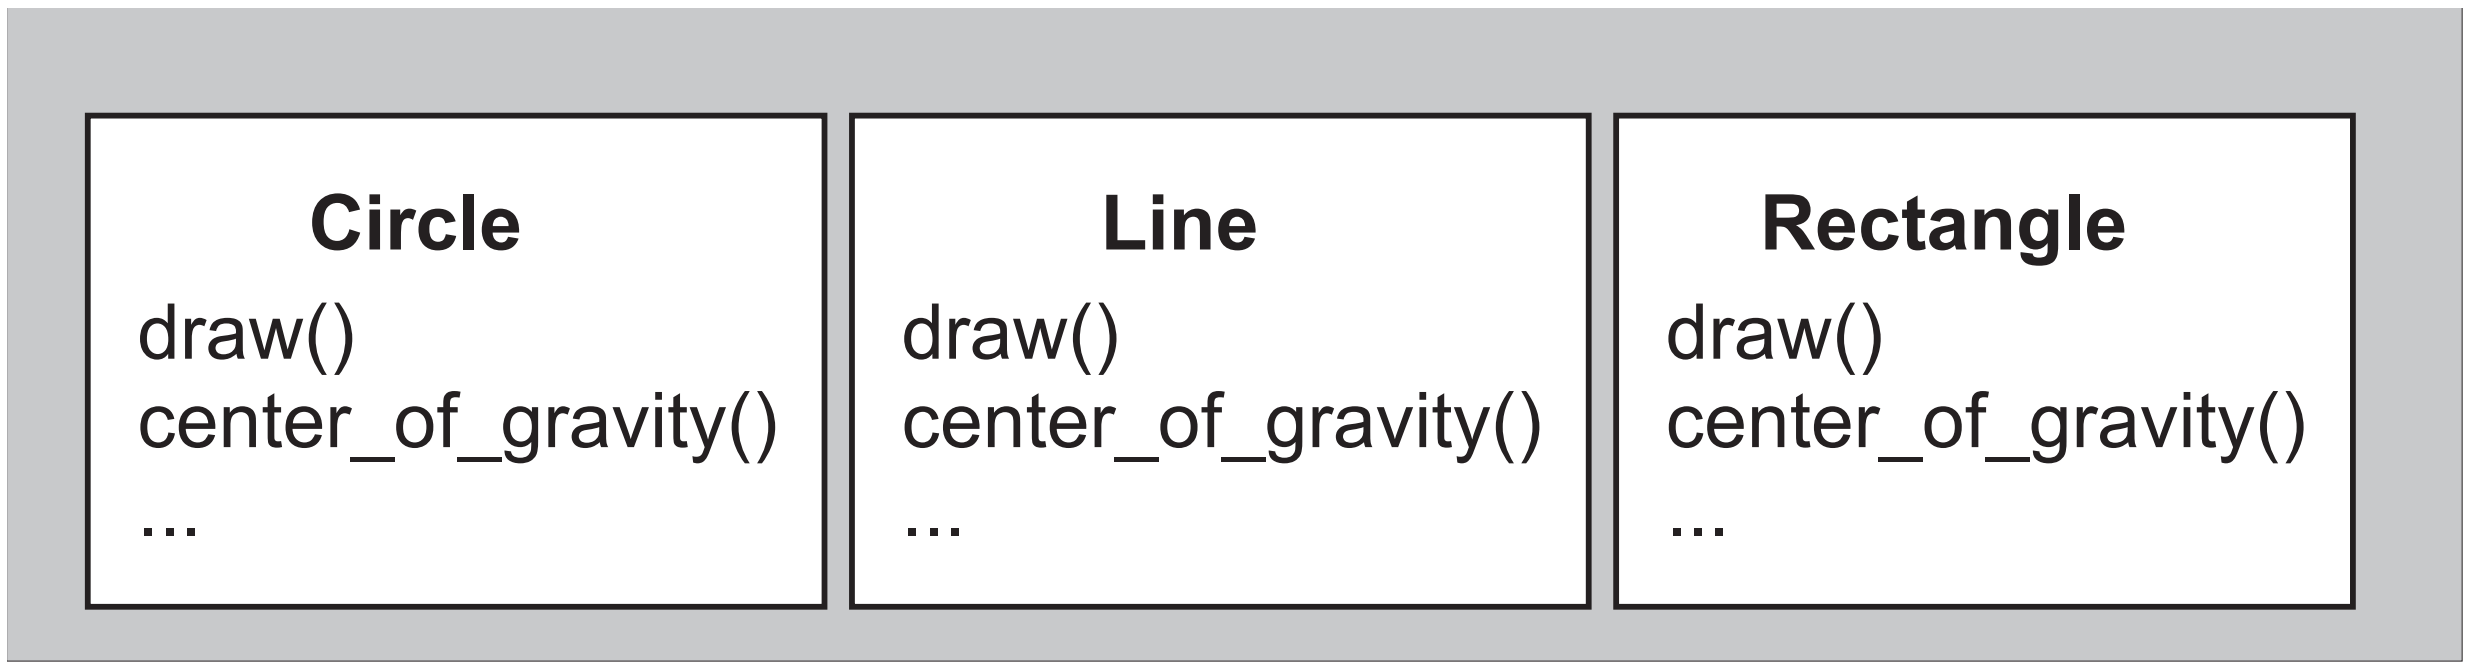
\includegraphics[width=0.8\textwidth]{content/3/chapter18/images/2.png} \\
Figure 18.2. Polymorphism implemented via templates
\end{center}

For example, the function myDraw() in the previous section:

\begin{lstlisting}[style=styleCXX]
void myDraw (GeoObj const& obj) // GeoObj is abstract base class
{
	obj.draw();
}
\end{lstlisting}

could conceivably be rewritten as

\begin{lstlisting}[style=styleCXX]
template<typename GeoObj>
void myDraw (GeoObj const& obj) // GeoObj is template parameter
{
	obj.draw();
}
\end{lstlisting}

Comparing the two implementations of myDraw(), we may conclude that the main difference is the specification of GeoObj as a template parameter instead of a common base class. There are, however, more fundamental differences under the hood. For example, using dynamic polymorphism, we had only one myDraw() function at run time, whereas with the template we have distinct functions, such as myDraw<Line>() and myDraw<Circle>().

We may attempt to recode the complete example of the previous section using static polymorphism. First, instead of a hierarchy of geometric classes, we have several individual geometric classes:

\hspace*{\fill} \\ %插入空行
\noindent
\textit{poly/statichier.hpp}
\begin{lstlisting}[style=styleCXX]
#include "coord.hpp"
// concrete geometric object class Circle
// - not derived from any class
class Circle {
	public:
	void draw() const;
	Coord center_of_gravity() const;
	...
};

// concrete geometric object class Line
// - not derived from any class
class Line {
	public:
	void draw() const;
	Coord center_of_gravity() const;
	...
};
...
\end{lstlisting}

Now, the application of these classes looks as follows:

\hspace*{\fill} \\ %插入空行
\noindent
\textit{poly/statichier.cpp}
\begin{lstlisting}[style=styleCXX]
#include "statichier.hpp"
#include <vector>

// draw any GeoObj
template<typename GeoObj>
void myDraw (GeoObj const& obj)
{
	obj.draw(); // call draw() according to type of object
}

// compute distance of center of gravity between two GeoObjs
template<typename GeoObj1, typename GeoObj2>
Coord distance (GeoObj1 const& x1, GeoObj2 const& x2)
{
	Coord c = x1.center_of_gravity() - x2.center_of_gravity();
	return c.abs(); // return coordinates as absolute values
}

// draw homogeneous collection of GeoObjs
template<typename GeoObj>
void drawElems (std::vector<GeoObj> const& elems)
{
	for (unsigned i=0; i<elems.size(); ++i) {
		elems[i].draw(); // call draw() according to type of element
	}
}

int main()
{
	Line l;
	Circle c, c1, c2;
	
	myDraw(l); // myDraw<Line>(GeoObj&) => Line::draw()
	myDraw(c); // myDraw<Circle>(GeoObj&) => Circle::draw()
	
	distance(c1,c2); // distance<Circle,Circle>(GeoObj1&,GeoObj2&)
	distance(l,c); // distance<Line,Circle>(GeoObj1&,GeoObj2&)
	
	// std::vector<GeoObj*> coll; // ERROR: no heterogeneous collection possible
	std::vector<Line> coll; // OK: homogeneous collection possible
	coll.push_back(l); // insert line
	drawElems(coll); // draw all lines
}
\end{lstlisting}

As with myDraw(), GeoObj can no longer be used as a concrete parameter type for distance(). Instead, we provide for two template parameters, GeoObj1 and GeoObj2, which enables different combinations of geometric object types to be accepted for the distance computation:

\begin{lstlisting}[style=styleCXX]
distance(l,c); // distance<Line,Circle>(GeoObj1&,GeoObj2&)
\end{lstlisting}

However, heterogeneous collections can no longer be handled transparently. This is where the static part of static polymorphism imposes its constraint: All types must be determined at compile time. Instead, we can easily introduce different collections for different geometric object types. There is no longer a requirement that the collection be limited to pointers, which can have significant advantages in terms of performance and type safety.


















